\begin{marginfigure}
	\setlength{\abovecaptionskip}{0.1pt plus 0.1pt minus 0.1pt}
	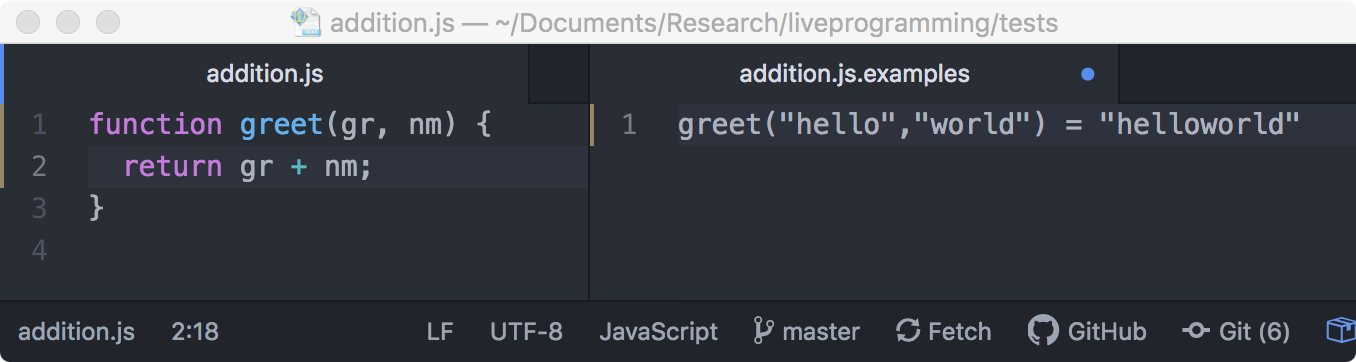
\includegraphics[width=0.55\textwidth]{figures/initial_greet}
	\caption{Code is written in the left hand panel,
	while examples are shown in the right hand panel.}
	\label{fig:init}
\end{marginfigure}
\begin{marginfigure}
	\setlength{\abovecaptionskip}{0.1pt plus 0.1pt minus 0.1pt}
	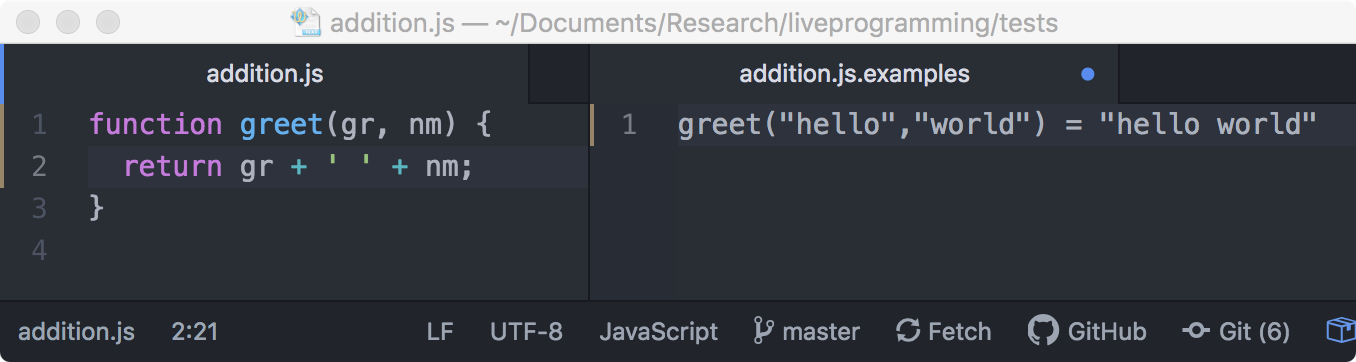
\includegraphics[width=0.55\textwidth]{figures/manual_change}
	\caption{When the code is modified, the examples update in real time.
	Here, the user has added a space to the output, by editing the code.}
	\label{fig:man_change}
\end{marginfigure}
\begin{marginfigure}
	\setlength{\abovecaptionskip}{0.1pt plus 0.1pt minus 0.1pt}
	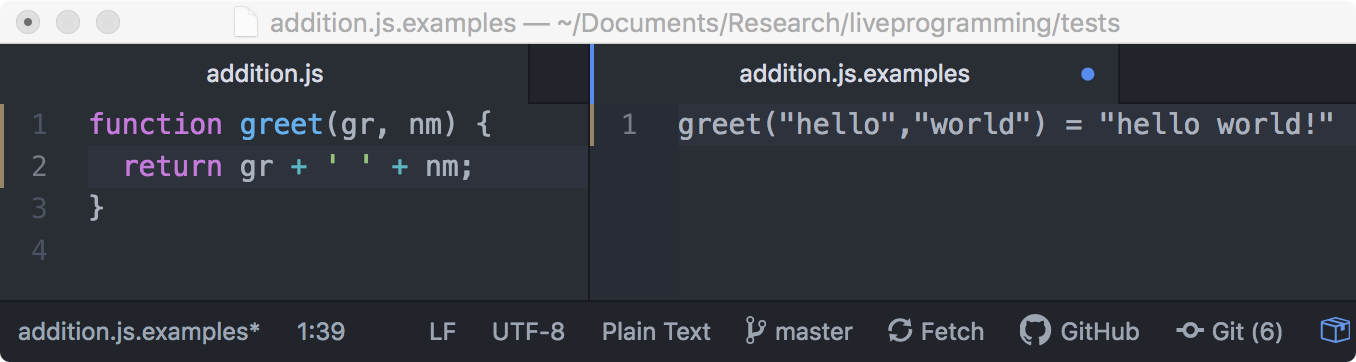
\includegraphics[width=0.55\textwidth]{figures/pbe_before}
	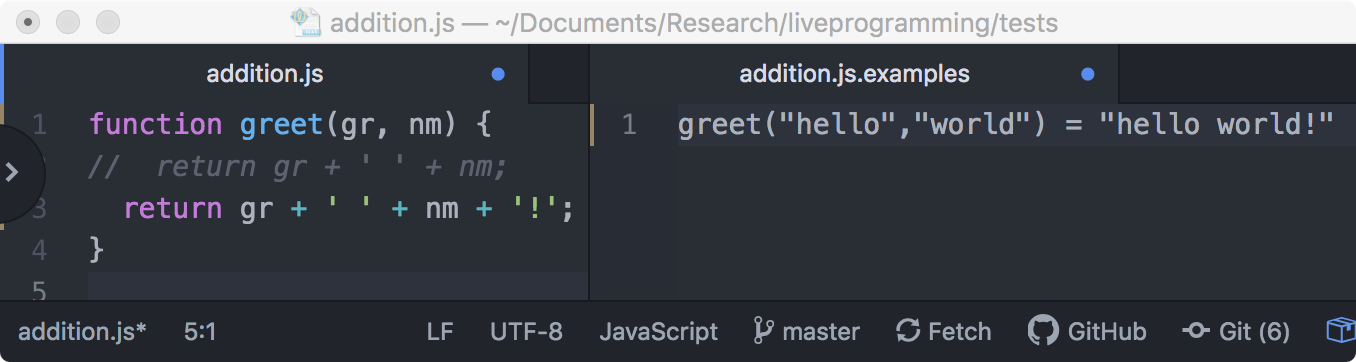
\includegraphics[width=0.55\textwidth]{figures/pbe_after}
	\caption{The user can also modify the output examples, to repair the code.  Here, the
	user has added a exclamation point to the end of the example's output, resulting in new code that appends an exclamation point.}
	\label{fig:pbe}
\end{marginfigure}

\section{Live Coding Plugin}
% We have implemented our live programming methodology as a plugin
% for Javascript programming in the Atom text editor~\cite{Atom}.
As shown in Figures~\ref{fig:init} to~\ref{fig:pbe}, our live programming methodology
relies on two panels.
Programmers write code in one panel.
The other panel displays input/output examples,
which are used for both live debugging,
and programming by example.
% The other panel displays input/output pairs for each function,
% which update in real time.
% By manipulating the displayed output value,
% the programmer can make use of PBE, to automatically update the code.

\subsection{Live Debugging}
We introduce \textit{live debugging} as a technique to show realtime feedback as programmers write code.
Programmers can specify an arbitrary number of function inputs.
As users write code, we continually run the code on the given inputs.By observing changes in the input-output pairs,
the user receives immediate feedback about whether the code is correct without actually analyzing it in detail.

As Javascript is an interpreted language, running syntactically correct code is fairly straightforward.
Unfortunately, the process of editing code often involves that code
being in a malformed, syntactically incorrect state.
Thus, we only update the displayed output when the code is, in fact,
syntactically valid.
When the user closes the file or editor,
we write the examples to a metadata file.
We reload the examples when the file is opened again.

\subsection{Programming by Example}
Our framework also allows for \textit{programming by example}~\cite{cypher93,lieberman01,synasc12}.
PBE  is a synthesis technique that automatically generates programs that coincide with given input/output examples. An example is specified as a tuple of input and output values. Given a set $S= \{(i_1, o_1),\ldots, (i_n, o_n)\}$ of input/output examples, the goal is to automatically derive a program $P$ such that for every $j$, $P(i_j) = o_i$. The success and impact of this line of work can be seen from the fact that some of this technology ships as part of the popular Flash Fill feature in Excel 2013~\cite{flashFillPOPL}.

When a user modifies an examples output, we update the code to reflect the change.
To synthesize code, we make use of CVC4's Syntax-guided synthesis (or SyGuS) algorithm~\cite{reynolds2017sygus}.
SyGuS is an approach that performs an enumerative search over the space of possible programs,
based on a given grammar.
We draw possible grammatical elements from the existing function implementation.
This both helps ensure that the newly generated code does not stray too far from the programmers original implementation,
and helps constraint the space CVC4 has to search over.
If we fail to find a solution to the SyGus problem, we iteratively increase the size of the grammar~\bill{Mark, more about how this is done?}.

\subsection{Overall design}
\bill{This seems like an important point to make somewhere, but I'm not sure this is the best place?}
Live debugging and programming by example naturally complement each other.
Programming by example makes use of examples as an easily readable and understandable specification. However, even if the synthesized program satisfies all the provided examples, it still might not correspond to the user's intentions. Examples are, by nature, an incomplete specification. However, since live debugging allows a programmer to immediately and continuously see the effects of changes, the user can provide new examples that better illustrate their intentions when synthesis fails. The synthesized program can then be refined with each new example. We call this approach {\emph{cooperative programming}}.

\subsection{Implementation}
We have implemented our live programming methodology as a plugin
for Javascript programming in the Atom text editor~\cite{Atom}.
To demonstrate the key ideas, our implementation supports live debugging for programs manipulating strings.
In the future, we plan to extend this support to other datatypes,
and we see no significant theoretical obstacles to doing so.